\section{Results}

\subsection{Null sanity check}

The publication-scale null experiment uses 5,000 paths per \(K\). At \(T=200\), observed crossing probabilities for the proposed method are \(0.0112\) (95\% CI \([0.0086,0.0145]\)) for \(K=24\) and \(0.0144\) (95\% CI \([0.0115,0.0181]\)) for \(K=32\). Oracle null crossing probabilities are \(0.0328\) and \(0.0324\), respectively. The strongest frozen-grid confidence-band benchmark has zero crossings in both null settings. These Monte Carlo estimates do not establish validity; they provide an implementation sanity check against the nominal anytime level \(\alpha=0.05\).

\subsection{Crossing probabilities}

Table~\ref{tab:crossing} summarizes the post-freeze publication-scale validation at \(T=200\).

\begin{table}[ht]
\centering
\caption{Crossing probability by \(T=200\) from 5,000 replications per condition. The confidence-band column reports the strongest ex-post configuration in the frozen grid.}
\label{tab:crossing}
\begin{tabular}{llccc}
\toprule
\(K\) & Condition & Static & Best band & Oracle\\
\midrule
24 & null & 0.0112 & 0.0000 & 0.0328\\
24 & \(\mathrm{Beta}(2,1)\) & 0.1824 & 0.0000 & 0.4258\\
24 & \(\mathrm{Beta}(4,1)\) & 0.8758 & 0.0106 & 0.9740\\
24 & \(\mathrm{Beta}(8,1)\) & 0.9980 & 0.3434 & 1.0000\\
32 & null & 0.0144 & 0.0000 & 0.0324\\
32 & \(\mathrm{Beta}(2,1)\) & 0.2036 & 0.0002 & 0.4396\\
32 & \(\mathrm{Beta}(4,1)\) & 0.9144 & 0.1152 & 0.9810\\
32 & \(\mathrm{Beta}(8,1)\) & 0.9998 & 0.8362 & 1.0000\\
\bottomrule
\end{tabular}
\end{table}

At the pre-specified primary point \(K=32,\gamma=4,T=200\),
\[
  \widehat P_{\mathrm{static}}=0.9144,\qquad
  \widehat P_{\mathrm{best\ grid}}=0.1152,\qquad
  \widehat P_{\mathrm{oracle}}=0.9810.
\]
The static 95\% Wilson interval is \([0.9063,0.9218]\). The paired static-minus-baseline gap is \(0.7992\) with 95\% bootstrap interval \([0.7880,0.8104]\), far above the frozen development margin of 0.15. The paired oracle-minus-static gap is \(0.0666\) with 95\% bootstrap interval \([0.0598,0.0736]\).

For the strong \(\gamma=8\) alternative at \(K=32\), static coupling reaches \(0.9998\), the oracle reaches \(1.0000\), and the strongest frozen-grid baseline reaches \(0.8362\). The smaller oracle-static gap is consistent with saturation under a strong signal.

For the weak \(\gamma=2\) alternative, static crossing probability is \(0.1824\) at \(K=24\) and \(0.2036\) at \(K=32\), while the oracle reaches \(0.4258\) and \(0.4396\). Unknown contamination identities therefore impose a substantial finite-reference penalty under weak shifts.

\begin{figure}[ht]
\centering
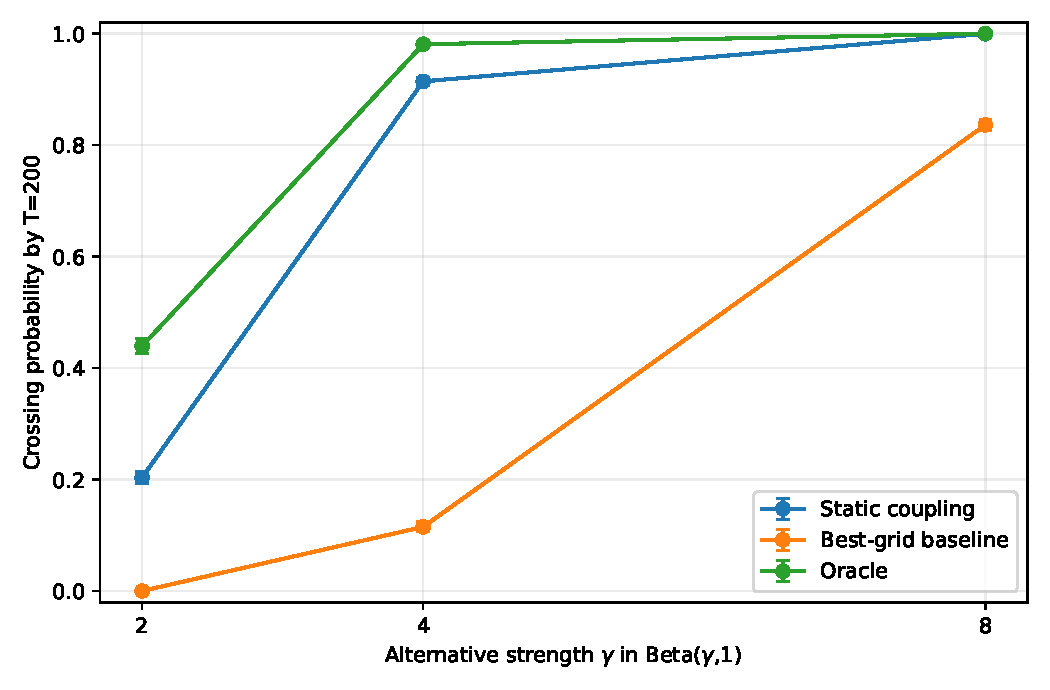
\includegraphics[width=0.82\linewidth]{../results/publication_v1/figures/crossing_T200_K32.pdf}
\caption{Crossing probability by \(T=200\) for \(K=32\), with 95\% Wilson intervals. The confidence-band curve is the strongest ex-post configuration from the frozen baseline grid for each alternative.}
\label{fig:crossing-k32}
\end{figure}

\subsection{Detection delays}

Table~\ref{tab:delays} reports median stopping times among paths that cross by \(T=200\).

\begin{table}[ht]
\centering
\caption{Median detected delay at \(T=200\).}
\label{tab:delays}
\begin{tabular}{llccc}
\toprule
\(K\) & Alternative & Static & Best grid & Oracle\\
\midrule
24 & \(\mathrm{Beta}(2,1)\) & 29 & -- & 17\\
24 & \(\mathrm{Beta}(4,1)\) & 20 & 117 & 9\\
24 & \(\mathrm{Beta}(8,1)\) & 8 & 75 & 5\\
32 & \(\mathrm{Beta}(2,1)\) & 22 & 178 & 16\\
32 & \(\mathrm{Beta}(4,1)\) & 15 & 97 & 8\\
32 & \(\mathrm{Beta}(8,1)\) & 7 & 53 & 4\\
\bottomrule
\end{tabular}
\end{table}

At the primary \(K=32,\gamma=4\) point, the proposed method has median detected stopping time 15 (95\% bootstrap CI \([14.5,16]\)), versus 97 \([92.5,102]\) for the best-grid baseline and 8 \([8,8]\) for the oracle. The \(\gamma=2\) baseline delays are not substantively comparable because the best-grid baseline crosses on zero of 5,000 paths for \(K=24\) and only one path for \(K=32\). Because these medians condition on detection, they are interpreted together with crossing probabilities rather than as standalone speed metrics.

\begin{figure}[ht]
\centering
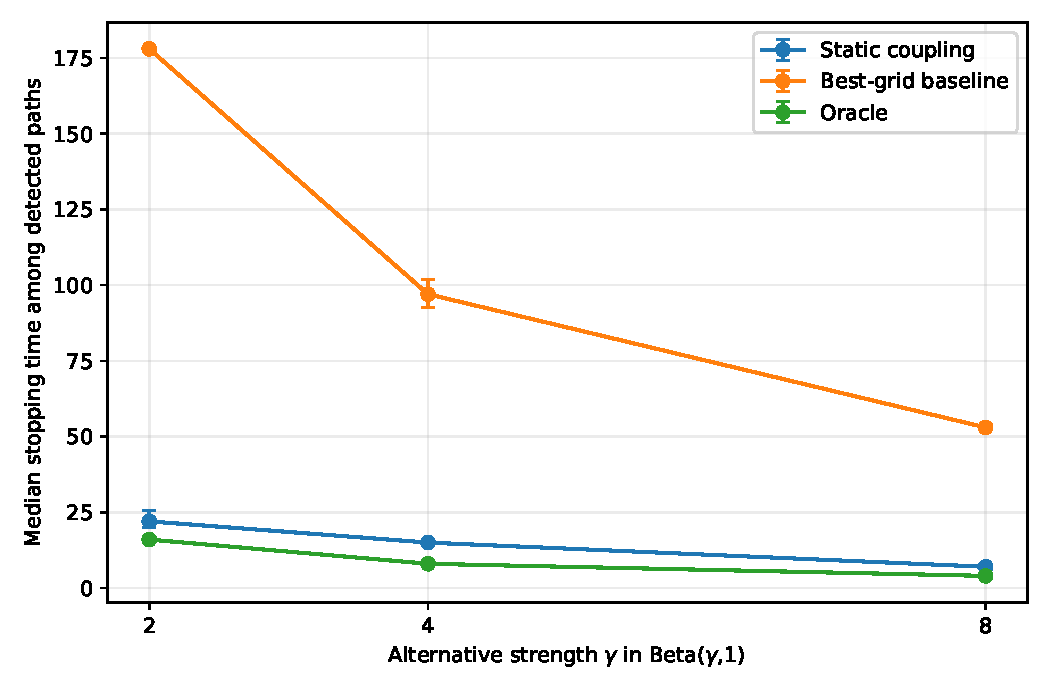
\includegraphics[width=0.82\linewidth]{../results/publication_v1/figures/delay_T200_K32.pdf}
\caption{Median stopping time among detected paths for \(K=32\), with bootstrap 95\% intervals. Delay is conditional on crossing and should be interpreted jointly with crossing probability.}
\label{fig:delay-k32}
\end{figure}

\subsection{Evidence diagnostics and tuning}

At \(K=32,\gamma=4,T=200\), median terminal log evidence is \(9.4131\) for static coupling and \(13.3054\) for the oracle. The selected best-grid comparator is the fixed band mixture at \(\delta=0.045\), with crossing probability \(0.1152\), median terminal log evidence \(-1.4528\), and threshold approximately 191.

At \(K=32,\gamma=8,T=200\), corresponding static and oracle median terminal log evidences are \(28.3517\) and \(34.3784\). The selected best-grid band mixture at \(\delta=0.045\) reaches crossing probability \(0.8362\) with median terminal log evidence \(20.1043\). These values are diagnostic only because the confidence-band thresholds differ from 20.

The selected baseline differs across conditions because the reported comparator is deliberately the strongest ex-post member of the frozen grid. This makes it a descriptive adversarial benchmark rather than one precommitted level-\(\alpha\) test.

The publication-scale run preserves the qualitative conclusions of the earlier 200-rep development audit without changing the method. Representative static crossing estimates move from \(0.880\) to \(0.8758\) for \(K=24,\gamma=4\), from \(0.935\) to \(0.9144\) for \(K=32,\gamma=4\), and from \(0.195\) to \(0.2036\) for \(K=32,\gamma=2\). Likewise, the \(K=32,\gamma=8\) best-grid baseline changes only from approximately \(0.840\) to \(0.8362\).

\subsection{Interpretation}

A confidence-band method asks which null CDFs remain compatible with the contaminated reference. Static coupling asks which \emph{single persistent set of contaminated identities} could explain the entire repeated rank history. The experiments suggest that preserving this persistent combinatorial constraint can retain substantially more usable finite-reference evidence, especially in the moderate-shift regime.
